% !TEX root = ../review.tex
\begin{frame}
\frametitle{Модель ошибок: общие сведения}
\begin{itemize}
  \item Было рассмотрено 3 датасета карт от BioNano
  \item С помощью RefAligner был построен референс
  \item Далее был проведён анализ ошибок
\end{itemize}
\end{frame}

\begin{frame}
\frametitle{Модель ошибок: ошибка в длине фрагмента}


\begin{figure}
\centering
\begin{minipage}{.5\textwidth}
  Валуев:
  \begin{gather*}
  e_k = \frac{o_k - r_k}{\sqrt{r_k}} \sim N(0, \sigma) \\
  o_k \sim N(r_k, \sigma^2 \, r_k)
  \end{gather*}
  \centering
  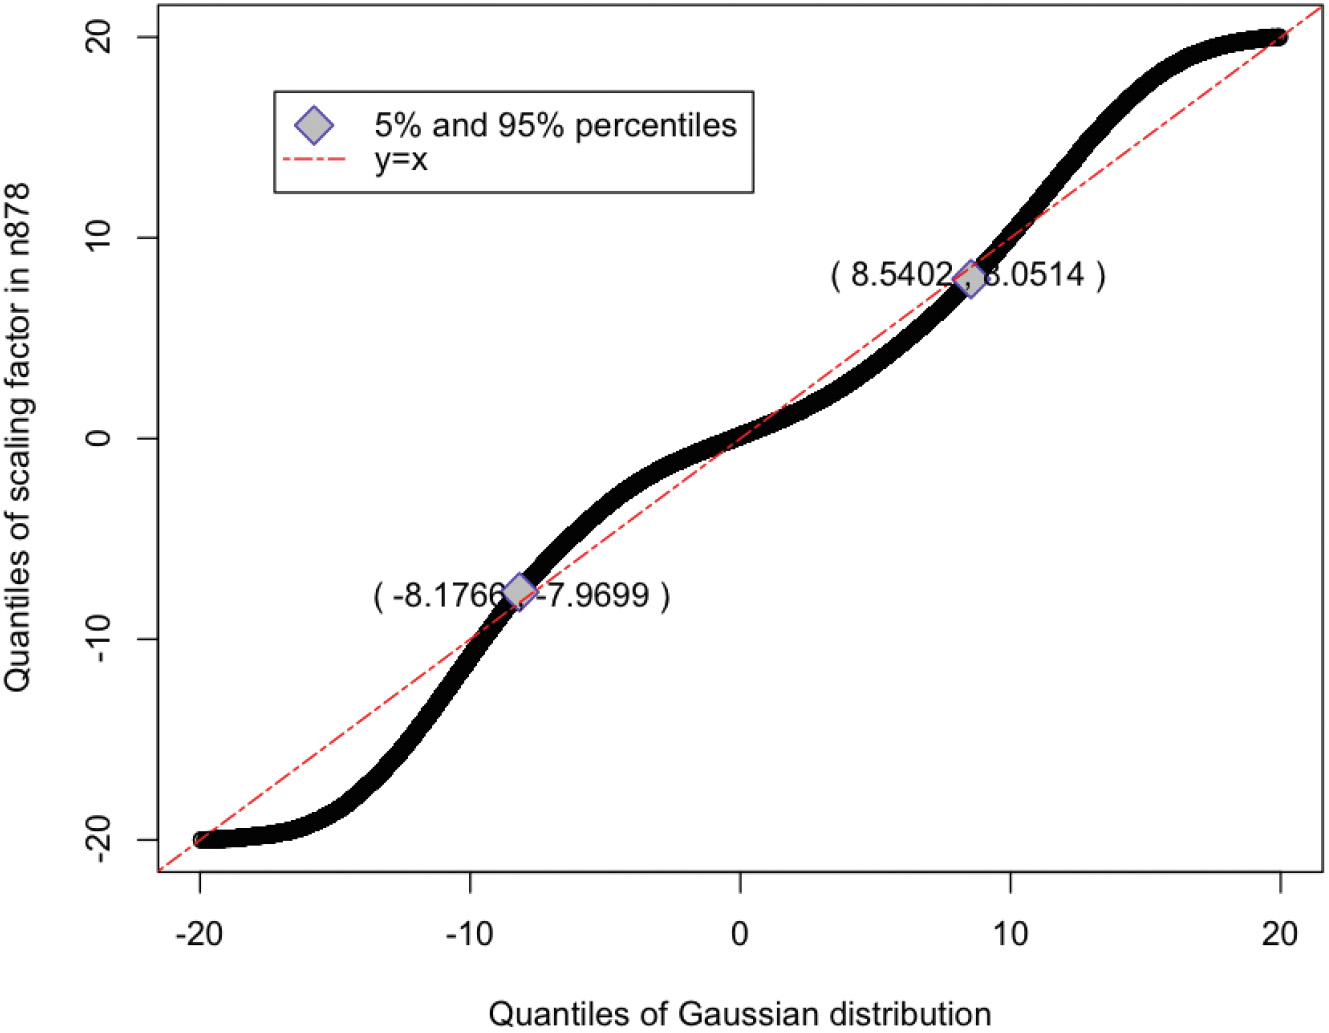
\includegraphics[width=.9\linewidth]{sigma_error_norm}
\end{minipage}%
\begin{minipage}{.5\textwidth}
  Новый подход:
  \begin{gather*}
  s_k = \frac{o_k}{r_k} \\
  s_k \sim Laplace(\mu, \beta)
  \end{gather*}
  \centering
  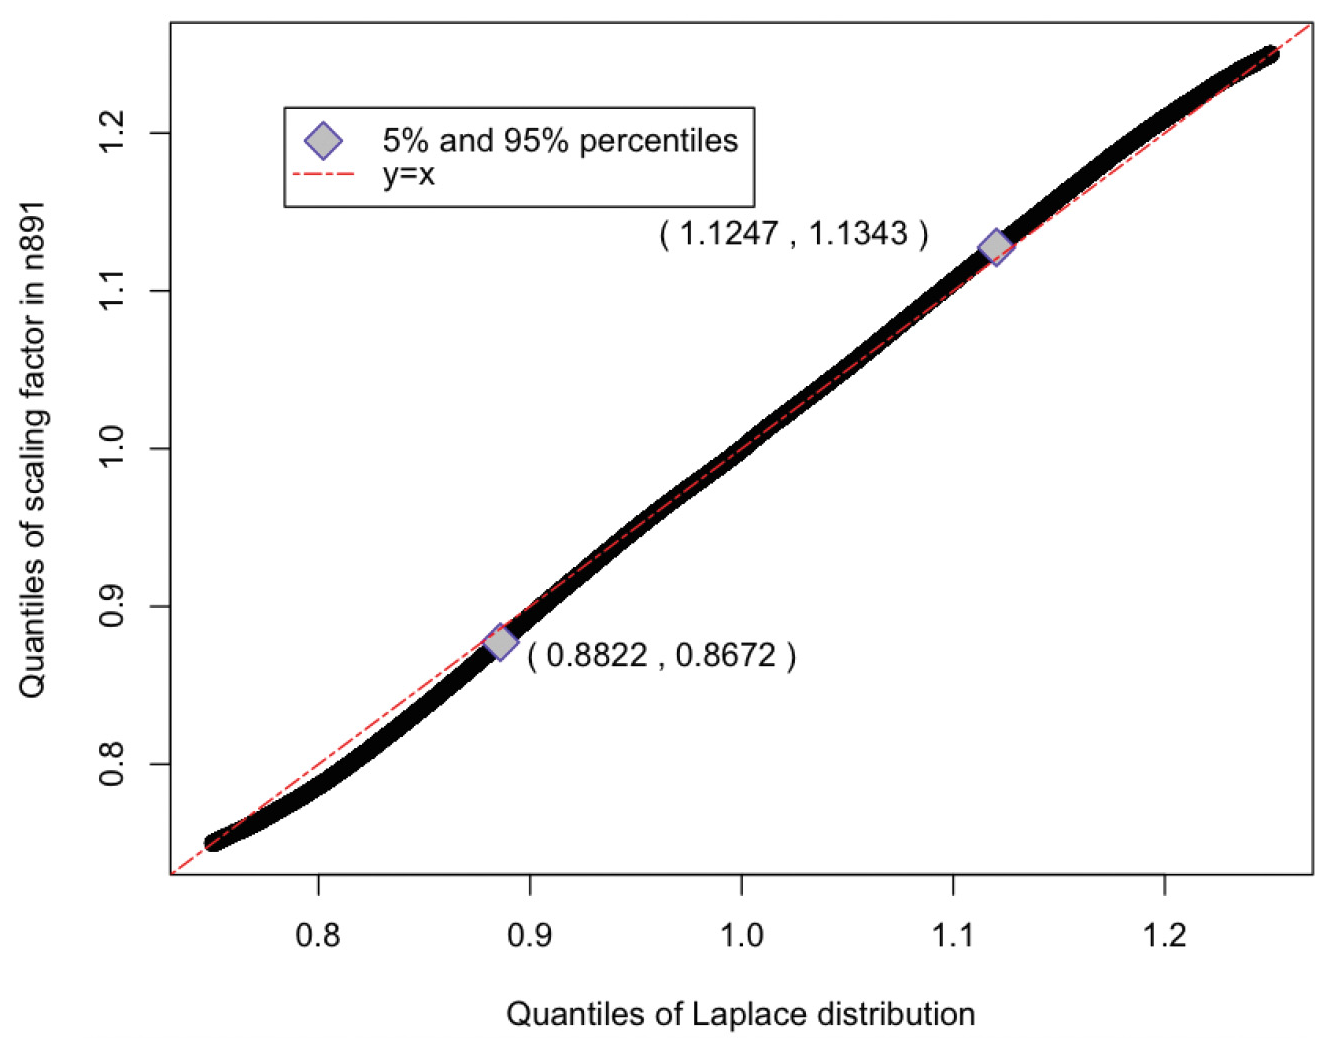
\includegraphics[width=.9\linewidth]{sigma_error_laplace}
\end{minipage}
\end{figure}
\end{frame}

\begin{frame}
\frametitle{Модель ошибок: пропущенные разрезы}

\end{frame}

\begin{frame}
\frametitle{Модель ошибок: лишние разрезы}

\end{frame}
